
\documentclass[a4paper,12pt]{article}

\usepackage{indentfirst}
\usepackage{makeidx}
\usepackage[pdftex]{graphicx}
\usepackage{wrapfig}
\usepackage[utf8]{inputenc}
\usepackage[english]{babel}
\usepackage{url}


%%
% New commands.

% Add an extra vertical space.
\newcommand{\espai}{\par\vspace{5mm}}

% How I do lists.
\newcommand{\mylist}{
\begin{itemize}
\setlength{\itemsep}{1pt}
\setlength{\parskip}{0pt}
\setlength{\parsep}{0pt}}
\newcommand{\mylistend}{\end{itemize}}

% Needed for the title.
\newcommand{\HRule}{\rule{\linewidth}{0.5mm}}

% So the links in the Table of Contents actually work.
\usepackage{hyperref}
\hypersetup{
  colorlinks,
  citecolor=black,
  filecolor=black,
  linkcolor=black,
  urlcolor=black
}


%%
% Hey! Ho! Let's go!


\begin{document}

% Title
% Copyright (C) 2014-2020 Miquel Sabaté Solà <mikisabate@gmail.com>
%
% This program is free software: you can redistribute it and/or modify
% it under the terms of the GNU General Public License as published by
% the Free Software Foundation, either version 3 of the License, or
% (at your option) any later version.
%
% This program is distributed in the hope that it will be useful,
% but WITHOUT ANY WARRANTY; without even the implied warranty of
% MERCHANTABILITY or FITNESS FOR A PARTICULAR PURPOSE.  See the
% GNU General Public License for more details.
%
% You should have received a copy of the GNU General Public License
% along with this program.  If not, see <http://www.gnu.org/licenses/>.


%%
% This file defines the title. It's created by hand by using the
% the instructions that were given in the following wiki page:
%       http://en.wikibooks.org/wiki/LaTeX/Title_Creation

\begin{titlepage}
\begin{center}

\textsc{\Large Barcelona School of Informatics}\\[0.5cm]

% Title
{ \small \HRule \\[0.4cm] }
{ \huge \bf Fita de seguiment \\[0.4cm] }
{ \small \HRule \\[0.4cm] }

% Author and supervisor
\begin{minipage}{0.4\textwidth}
\begin{flushleft} \large
\emph{Author:}\\
Miquel \textsc{Sabaté Solà}
\end{flushleft}
\end{minipage}
\begin{minipage}{0.4\textwidth}
\begin{flushright} \large
\emph{Director:} \\
Jordi \textsc{Garcia Almiñana}
\end{flushright}
\end{minipage}

\vfill

% Bottom of the page
{\large \today}

\end{center}
\end{titlepage}


\tableofcontents
\thispagestyle{empty}

\setcounter{page}{1}

% Introduction.
\newpage
% Copyright (C) 2014-2015 Miquel Sabaté Solà <mikisabate@gmail.com>
%
% This program is free software: you can redistribute it and/or modify
% it under the terms of the GNU General Public License as published by
% the Free Software Foundation, either version 3 of the License, or
% (at your option) any later version.
%
% This program is distributed in the hope that it will be useful,
% but WITHOUT ANY WARRANTY; without even the implied warranty of
% MERCHANTABILITY or FITNESS FOR A PARTICULAR PURPOSE.  See the
% GNU General Public License for more details.
%
% You should have received a copy of the GNU General Public License
% along with this program.  If not, see <http://www.gnu.org/licenses/>.

\section{Introduction}

\subsection{Context}

This is the final report of the GEP course. The GEP course is part of my
Bachelor Degree Thesis, and consists of a set of deliveries and instructions
that has helped me in the preparation of my Thesis.

My Bachelor Degree Thesis is being presented at the Barcelona School of
Informatics and is directed by Mr. Jordi García Almiñana. The project was
originally envisioned by the director, and the author must develop a solution
for the given problem.

\subsection{Brief project description}

My Bachelor's Degree Thesis is about building an infrastructure that is
capable of providing a set of services from the data that has been collected
and processed. This data will come from initiatives like OpenData BCN and
iCity. This infrastructure will fetch and process all this data in realtime,
by using a set of new technologies that allow us to do so.

\subsection{Brief state of the art}

Since the appearence of the MapReduce algorithm, a lot of different
technologies have evolved so we can now fetch and process huge amounts of data.
This is important for the computer industry, but also for governments and other
associations.

We have a huge list of technologies that deal with Big data, but maybe the more
important ones are Hadoop and Storm. Storm is the base technology that I will be
using in this project. It's a modern and mature framework that will allow me to
build a realtime pipeline that is capable of fetching and processing huge
amounts of data.

\subsection{Purpose}

The purpose of this project is to provide a base infrastructure capable of
fetching and processing large amounts of data from iniciatives like OpenData
BCN and iCity to provide a set of services improving the actual situation.


% Scope of the project.
\newpage

\section{Project scope}

\subsection{The context: Big data and streaming}

Once upon a time, Google released a paper called: ``MapReduce: Simplified Data
Processing on Large Clusters''\cite{mapreduce}. This was the beginning of
a revolution in the data processing front. After that, lots of efforts
have been put in this direction, being Hadoop one of the most important
accomplishments. Hadoop (and related technologies) has made it possible
to store and process data at scales previously unthinkable.

However, these technologies have one major drawback: they are not realtime
systems, nor are they meant to be. In order to solve this issue one has to
manually implement a network of queues and workers. These workers would
eventually send messages, update databases, and send new messages to other
queues for further processing. This, of course, has some serious limitations:
it's tedious, it doesn't scale, and it has little fault-tolerance.

In order to fix the previously cited issues from the core, some projects like
Yahoo! S4 and Twitter Storm emerged. Both projects have some differences but
they have a clear focus: to ease the writing of parallel realtime computation.
Sadly, nowadays the S4 project is dead. This is why in this thesis I'm picking
Storm\cite{storm} as the base technology (plus, the Storm project has a very
active community).

\subsection{My proposal}

My Bachelor Degree Thesis is about building an infrastructure that is capable
of providing a set of services from the data that has been collected and
processed. The raw data for this infrastructure will come from OpenData
BCN\cite{opendata} iniciative. That is, the infrastructure that I'm going
to build for my thesis will provide additional features to the OpenData
BCN iniciative that are only possible by building a cluster that will
process data continiously.

This infrastructure will fetch and process all this data in realtime, using
Storm as the base technology in the software front. This is important because
the users of all the services build upon these infrastructure will be able to
fetch all the processed data also in realtime.

This means that I am not just going to do research only in the Big data and
streaming front, but I'm also going to research more deeply in the whole concept
of ``Smart City''. This is because this infrastructure will be built in a way
so other services can fetch our processed data to improve, promote and have a
better understanding of the city of Barcelona.

This is my proposal. However, any proposal is doomed if it's not specified a set
of rules that define the scope of it. The scope of my Thesis will consist of
the following points:

\mylist
  \item Design a cluster that can match our requirements.
  \item Design a base system that will fetch and process all the data.
  \item Provide a couple of useful services on top of the base system.
\mylistend

\subsection{Goals}

The previous section contained all the information regarding what my Thesis is
about. Now I am going to relate my goals for doing this project.

\mylist
  \item {\bf Research}. Because of this thesis, I will be doing a lot of
research. My main focus will be: Big data, streaming processing and smart
cities. I will be investigating, for each of them, their state of the art, what
should we know about and what can we do with them.
  \item {\bf Learn} some technologies as a side effect. My base technology will
be the Storm framework. This means that I will be learning and improving my
skills in programming languages like Java and Scala. I will also be improving my
skills with concurrent programming. I will further also my knowledge on hardware
by analyzing what kind of machines we need in order to provide and scale all the
services.
  \item {\bf Provide} a useful technology base. The main goal of this Thesis is
to create a base technology that will be useful to other people. This way we
will be able to provide a set of services that will potentially improve the
city of Barcelona on multiple ways. I am really optimistic about this project,
and I can see other thesis from other students about improving or extending the
infrastructure that I'll be building in my thesis.
  \item {\bf Practice}. The Bachelor Degree Thesis is the final stop of this
journey that I've been doing in the Barcelona School of Informatics. I've
learnt a lot and I am ready to apply some of the concepts learnt in this
university to this Thesis.

\mylistend

\subsection{About the development}

Lastly, I want to clarify how I want to develop this project. First of all, the
code that will make all this to happen is open source. This means that all of
the base technology and the code that I will be developing is all open source.
In fact, all my code is hosted on
Github\footnote{https://github.com/mssola/thesis}. This is really important for
me for the following reasons:

\mylist
  \item I am a strong advocate of Open Source.
  \item It could help future thesis based on this infrastructure.
  \item It could help anyone in the world that is developing something similar.
  \item It is fair.
\mylistend

My workflow will consist in discussing any doubts that I would have with my
teacher and keep on developing the whole platform in an open way. Finally, I
want to point out my resources, that I quite humble. I will spend most of my
time doing this project, with all the resources that I have.


% Schedule
\newpage

\section{Planning}

\subsection{Project planning and feasability}

The first period of the project is dedicated to studying the feasability of the
project and to do the initial planning of the project. This is done through a
course called GEP, that is currently running. This course includes the
following stages:

\mylist
  \item Scope of the project.
  \item Project planning.
  \item Budget and sustainability.
  \item Preliminary presentation.
  \item Bibliography.
  \item List of conditions.
  \item Oral presentation and delivery of the final document.
\mylistend

\subsection{Project analysis and design}

The main goal of this stage is to draw a clear picture of the project and
analyze all the goals of the project. After doing this, I will move my efforts
towards the design of the application.

Therefore, this stage is made out of two sub stages. The first one, the
analysis of the project. In this sub stage I will be defining all the goals,lose
requirements, features and use cases of my application.

The other sub stage consists in design the application. This will be done by
creating diagrams, drawing flow charts, etc.

\subsection{Project iterations}

\begin{enumerate}
 \item {\bf Development of the core software infrastructure}

 In this iteration I am going to focus on the core infrastructure that has to
hold the whole application. This will be executed only in the software front.
I will consider that this stage has ended when there is production-ready base
software that can hold the infrastructure and that is well documented and
thoroughly tested.

 \item {\bf Providing services}

 The next iteration consists of building services on top of the base
infrastructure that has been created in the previous stage. Similarly to the
previous stage, all the services build at this point will be documented and
tested consciously.

  \item {\bf Designing the cluster}

  At this point, we have the software ready to be put in production. Now we
need to design and implement a cluster that can hold the software. In this
stage I will be using lots of concepts learnt at the university, specially from
the CPD course.

  \item {\bf Concluding the development}

  In the last iteration I will be concluding the development of this project.
It consists of doing final tests on both the software and the hardware. This
last iteration will be used to make sure that everything runs smoothly.
\end{enumerate}


\subsection{Final stage}

The final stage consists on closing the project. Since all the code and the
cluster design has already been set up to this point, I am just going to focus
on the following topics:

\mylist
  \item Documentation.
  \item Final report.
  \item Final presentation.
\mylistend

\section*{Gantt chart}

\begin{center}
  \hspace*{-2cm}
  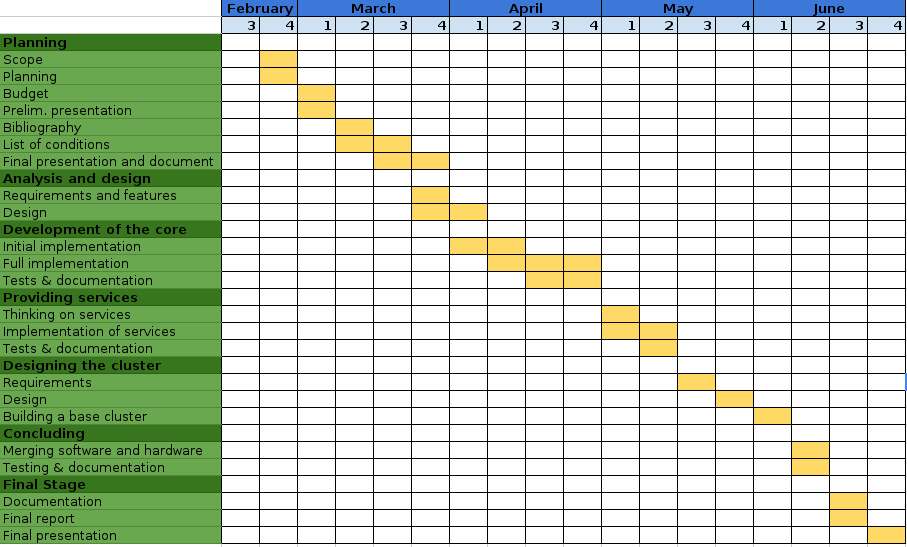
\includegraphics[scale=0.75]{images/gantt.png}
\end{center}

I don't like to compute the work to be done in hours. I prefer to do it in
weeks. In the Gantt chart we can see the scheduling that I've made for the
project divided by weeks. Some tasks are overlapping in some weeks. This is
quite normal.

The total amount of hours is not fixed, it depends on the work that is needed
to be done for each task. The important thing here is that we make the
deadlines with no problems.

\subsection{Action plan}

At this point, it is clear how the stages are scheduled. Now, what happens if
any stage has a different duration than expected ? In my case, I will just
start the next stage. That is, if I will start each stage as soon as possible.

In the end of each stage I will do an evaluation of the work done so far. This
will allow me to rearrange the schedule so I don't lose the track of the
development of the project.

Moreover, at the end of each iteration I will meet with my director to analyze
how is the project going. This will force me to work hard to meet the deadlines
and it will also give me the oportunity to have some feedback from the director.


% Budget
\newpage

\section{Budget}

\subsection{Introduction}

In this delivery I am focusing on the budget and on the impact of my project.
First of all, I am going to focus on the budget. This includes doing some math
in the following topics: human resources, hardware and software.

Lastly, I will be explaining the impact that I expect that this project will
have. My only considerations for the impact will be the social impact and the
environmental impact.

\subsection{Budget}

In this section I will be describing the estimated costs that this project will
have. After specifying each of the costs, I will make up a total amount of
estimated costs. This will lead me to conclude the needed budget for this
project.

\subsection{Human resources}

What I want to do in this section is to describe all the costs related to
employing people to develop this project.

Luckily enough, it is just me in this project, so I just have to compute my own
salary. After doing some research, I have found that the average salary for a
Big data analyst is around 99,000 USD a year. This boils down to 51 USD per
hour. I did my scheduling based on weeks, instead of hours, and I think that I
will spend 20 hours in average per week. This means that in total, my salary
during the project will be:

\[
  20\ hours \cdot 16\ weeks \cdot 51\ USD = 16,320\ USD
\]


\subsection{Hardware}

Ideally in this section I would explain all the costs regarding the hardware.
However, I can't compute this because the only hardware that I will specify will
be the cluster which, in turn, is just a proposal. Other things like my laptop
won't be counted in this section They are not a cost for this project since I
use them for personal purposes too.

\subsection{Software}

In this section I will describe all the costs associated with software. In
short, this is my budget for software:

\[
  0\ \$
\]

All the software that I will be using for this project is free: both as in
``free beer'' as in ``free speech''. There are no fees for any license, I won't
be using any paid service, etc. Nothing.

\subsection{Total}

The main conclusion is that the only cost associated to this project is just my
salary. Therefore, my estimated costs are a total of \$16,320.

\subsection{Social impact}

This section is really important for this project. It is about the impact that
this platform will make to society. This is not a direct impact, but an
indirect one. The social impact of this platform comes in two ways:

\mylist
  \item The fact that a number of businesses will take advantage that this
platform exists.
  \item Indirectly, all the impact that all the services built on top of this
platform will produce.
\mylistend

This means that, ideally, the social impact of this platform can be huge.

\subsection{Environmental impact}

In the same way that this platform can bring a lot of goodness in the social
front, it certaintly comes with a cost. In my case the cost is an environmental
impact that cannot be understated.

In this project I will propose an ideal cluster that would be able to run the
software that I will design. The problem here is that maintaining a cluster
means the following:

\mylist
  \item Power supply.
  \item Maintaining a cooling system.
  \item The implied environmental costs of building the cluster.
\mylistend

All of these can be reduced by using the minimum amount of cluster time as
possible. This means to run the software in ``batches'' or with a very low
latency. However, this is not possible at all if the cluster has a lot of
requests, and that is to be expected.

Therefore, in the development of the cluster I will focus most of my efforts
into keeping the cluster as environmental friendly as possible.


% Biblio
\newpage
% Copyright (C) 2014 Miquel Sabaté Solà <mikisabate@gmail.com>
% This file is licensed under the MIT license.
% See the LICENSE file.

\section{Bibliography}

\subsection{Context}

This section aims to describe the context within which the project will be
developed. We differntiate between: developers, the tutor, library developers
and the users.

\subsection{Developers}

I am the only developer of this project. I will make use of my knowledge on the
topic, the guidance of my tutor and the previous work of the library developers
to accomplish my goals.

\subsection{Tutor}

Jordi García Almiñana is my tutor. His role is to make sure that I
have both my focus and my goals straight. He will be guiding me through the
development of this project and giving me some tips of advice.

\subsection{Library developers}

Library developers are all the developers that have contributed to the
libraries that I will be using to build this project. There are a lot of
developers, coming from different backgrounds and goals.

\subsection{Users}

The users are everyone that will make use of this project. We can distinguish
different users:

\mylist
\item End users that will make use of the data generated from our platform.
\item Developers that will make use of our services.
\item Developers that will read the code of this project, so they can get a
benefit from it.
\mylistend

\subsection{State of the art}

In this section I will be describing the state of the art. That is, I will
describe what is the current situation, the problems arising, and solutions
from other developers.

\subsection{Big data}

Big data\cite{wikibigdata} is a term that has been coined lately. Big data is
the term for a collection of data sets so large and complex that it becomes
difficult to process using on-hand database management tools or traditional
data processing applications.

Big data is difficult to work with using most relational database management
systems and desktop statistics and visualization packages, requiring instead
``massively parallel software running on tens, hundreds, or even thousands of
servers''. The definition of Big data varies depending on the organization.

\subsection{Map Reduce}

Since we cannot perform operations on Big data on a traditional way, we have to
build tools that will tackle this problem accordingly. The first step was made
by Google with its ``MapReduce'' algorithm\cite{mapreduce}. The MapReduce
algorithm solves this problem by mapping a specified problem (e.g. a file with
data inside of it) and finally reducing the results back. This is an easy way
to distribute the work on different machines, so they are as efficient as
possible.

Multiple implementations of MapReduce arised after the announcement of
MapReduce. The most famous implementation being Hadoop\cite{hadoop}. Hadoop
implements the algorithm of MapReduce with fault tolerance. It also provides
the idea of HDFS (Hadoop File System), a distributed file system.

\subsection{Streaming}

At this point, it is clear that Hadoop and the MapReduce algorithm brings a lot
of advantages and opportunities. This is nice but Hadoop does not do one thing:
realtime operations. Hadoop and similar technologies are not realtime systems,
nor are they meant to be. Hadoop is not designed to be a realtime system, and
thus any effort to hack Hadoop in any realtime direction is a waste of time.
This is because realtime data processing has a fundamentally different set of
requirements than batch processing.

This is really a problem, because realtime data processing at massive scale is
becoming more and more of a requirement these days for businesses. To fill this
hole, technologies such as Yahoo! S4 and Twitter Storm\cite{storm} were
developed. Right now Yahoo! S4 is more or less abandoned and Twitter Storm is
really alive, but under the umbrella of the Apache foundation\cite{apache} This
is why my project will be based on Storm.

Before Storm, you would typically have to manually build a network of queues and
workers to do realtime processing. Workers would process messages off a queue,
update databases, and send new messages to other queues for further processing.
Unfortunately, this approach has serious limitations:

\mylist
\item {\bf Tedious}: You spend most of your development time configuring where to send
messages, deploying workers, and deploying intermediate queues. The realtime
processing logic that you care about corresponds to a relatively small
percentage of your codebase.
\item {\bf Painful} to scale: When the message throughput get too high for a single worker
or queue, you need to partition how the data is spread around. You need to
reconfigure the other workers to know the new locations to send messages. This
introduces moving parts and new pieces that can fail.
\mylistend

Apart from Storm, I will make use of other technologies such as
Summingbird\cite{summingbird} and other technologies from Twitter\cite{twitter}
and Yahoo\cite{yahoo}. These two companies have open sourced a lot of libraries
for Storm that will be useful in the development of this project.

\subsection{Future}

The future of Big data will be tied in the future to the streaming
technologies. They solve increasingly important issues and they perform efficiently
when dealing with lots of data.

It's clear, then, that more companies will follow this lead. This implies more
support and more libraries available out there.

\subsection{Smart cities}

Finally, I would like to talk about the concept of Smart Cities\cite{smart}.
Smart cities is a new concept that embodies all the efforts to make cities more
efficient and more reliable.

That key component are IT technologies. We use data centers, sensors, etc. to
compute key elements. With all the computed data, we can then analyze which
parts of the cities can be improved in order to make citizens happier and
services more efficient.

\newpage

\renewcommand\refname{Bibliography}
\begin{thebibliography}{9}

\bibitem{wikibigdata}
  Dan Kusnetzky,
  {\emph What is Big Data?}.
  \url{http://www.zdnet.com/blog/virtualization/what-is-big-data/1708}",
  2010.

\bibitem{mapreduce}
  Jeffrey Dean and Sanjay Ghemawat,
  {\emph MapReduce: Simplified Data Processing on Large Clusters}
  2004.

\bibitem{hadoop}
  Hadoop. Wikipedia.
  \url{http://en.wikipedia.org/wiki/Hadoop}

\bibitem{storm}
  Storm.
  \url{http://storm.incubator.apache.org/}

\bibitem{apache}
  Apache Software Foundation.
  \url{http://www.apache.org/}

\bibitem{summingbird}
  Github page for Summingbird.
  \url{https://github.com/twitter/summingbird}

\bibitem{smart}
  Smart Cities.
  \url{http://en.wikipedia.org/wiki/Smart_cities}

\bibitem{twitter}
  Github page of Twitter.
  \url{https://github.com/twitter}

\bibitem{yahoo}
  Github page of Yahoo!.
  \url{https://github.com/yahoo}

\bibitem{opendata}
  OpenData BCN webpage.
  \url{http://opendata.bcn.cat/opendata/en}

\end{thebibliography}


\end{document}
